\section{Latar Belakang}
\par Robot Line Follower tanpa menggunakan PID akan menunjukkan penyimpangan yang amat besar \cite{nath2013implementation}. Hal tersebut akan mempengaruhi kinerja seperti proses pemindahan barang.Dalam suatu instansi, biaya untuk praktisi tergantung pada layanan yang diberikan \cite{punetha2013development}. Sama halnya seperti pada proses logistik semua personil harus bekerja secara profesional. Bagaimana hal tersebut dapat mempengaruhi baik-buruknya pelayanan.
\section{Tujuan dan Manfaat}

\section{Alat}
\begin{enumerate}
  \item Arduino UNO seperti pada gambar \ref{fig:arduinouno},
  \begin{figure}[!htbp]
  \centering
  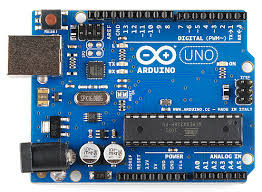
\includegraphics[width=.75\textwidth]{figures/Arduino/arduinouno.jpg}
  \caption{Ini adalah Arduino UNO}\label{fig:arduinouno}
\end{figure}
  \item Kabel Jumper seperti pada gambar \ref{fig:jumper},
  \begin{figure}[!htbp]
  \centering
  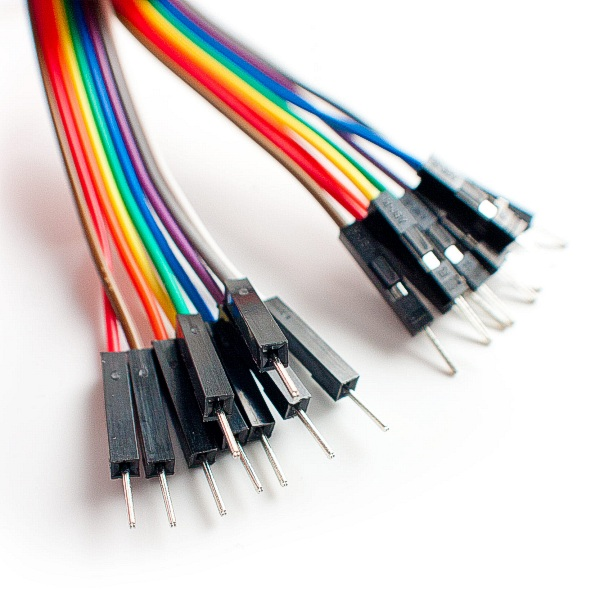
\includegraphics[width=.75\textwidth]{figures/Arduino/jumper.jpg}
  \caption{Ini adalah Kabel Jumper}\label{fig:jumper}
\end{figure}
  \item Breadboard seperti pada gambar \ref{fig:breadboard},
  \begin{figure}[!htbp]
  \centering
  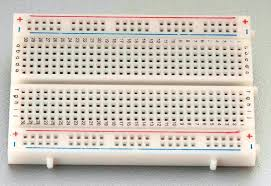
\includegraphics[width=.75\textwidth]{figures/Arduino/breadboard.jpg}
  \caption{Ini adalah Breadboard}\label{fig:breadboard}
\end{figure}
  \item
  \item \textit{Coming Soon}
\end{enumerate}

\section{Software Pendukung}
\subsection{Simulator}
Sebelum memulai merangkai ada baiknya untuk merancang terlebih dahulu. Perancangan dilakukan agar dapat menganalisa kebutuhan baik itu perangkat keras maupun script code pendukung. Ada beberapa simulator yang dapat digunakan secara gratis misalnya VBB (Virtual Bread Board), Proteus dll. Untuk perancangan Line Follower Robotic akan menggunakan VBB.
\subsubsection{VBB (Virtual Bread Board)}


\subsection{IDE}
IDE adalah sebuah software yang berperan untuk menulis program, meng-compile menjadi kode biner dan meng-upload ke dalam memory microcontroller. Ada banyak projek dan alat-alat dikembangkan oleh akademisi dan profesional dengan menggunakan Arduino, selain itu juga ada banyak modul-modul pendukung (sensor, tampilan, penggerak dan sebagainya)yang dibuat oleh pihak lain untuk bisa disambungkan dengan Arduino. Arduino berevolusi menjadi sebuah platform karena ia menjadi pilihan dan acuan bagi banyak praktisi \cite{djuandi2011pengenalan}.

\section{Langkah-langkah}
\subsection{Installasi Software}
\begin{enumerate}
  \item Installasi VBB(\textit{Virtual Bread Board})
    \begin{enumerate}
        \item Download installer vbb
        \item Double-click installer vbb,seperti pada gambar \ref{fig:installer}
            \begin{figure}[!htbp]
            \centering
            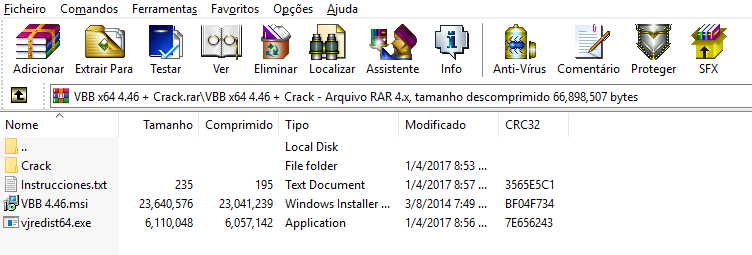
\includegraphics[width=.75\textwidth]{figures/VBB/installer.png}
            \caption{Ini adalah installer}\label{fig:installer}
            \end{figure}
        \item Maka akan tampil seperti gambar \ref{fig:halawalinstallasi}
            \begin{figure}[!htbp]
            \centering
            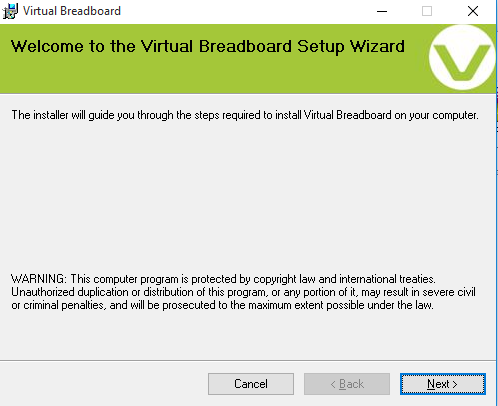
\includegraphics[width=.75\textwidth]{figures/VBB/halawalinstallasi.png}
            \caption{Ini adalah Halaman Awal Installasi}\label{fig:halawalinstallasi}
            \end{figure}
        \item Pilih direktori penyimpanan seperti gambar \ref{fig:memilihdirektori}
            \begin{figure}[!htbp]
            \centering
            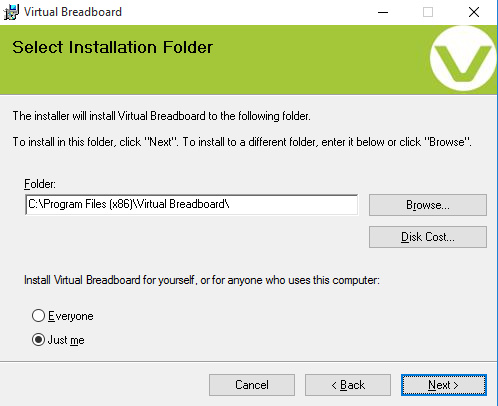
\includegraphics[width=.75\textwidth]{figures/VBB/memilihdirektori.png}
            \caption{Ini adalah Halaman Pemilihan Direktori}\label{fig:memilihdirektori}
            \end{figure}
        \item Kemudian tekan tombol next, maka akan muncul halaman konfirmasi seperti pada gambar \ref{fig:konfirmasiinstall}
            \begin{figure}[!htbp]
            \centering
            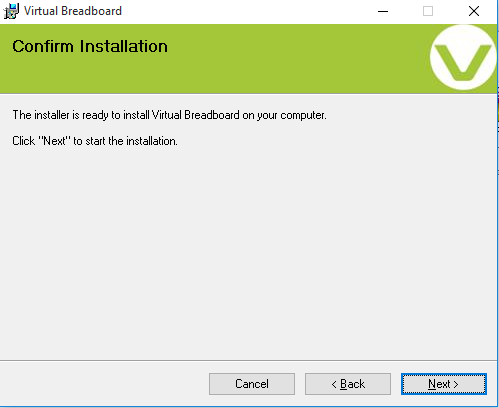
\includegraphics[width=.75\textwidth]{figures/VBB/konfirmasiinstall.png}
            \caption{Ini adalah Halaman Konfirmasi Installasi}\label{fig:konfirmasiinstall}
            \end{figure}
        \item Lalu tunggu sampai proses installasi selesai, seperti pada gambar \ref{fig:prosesinstallasi}
            \begin{figure}[!htbp]
            \centering
            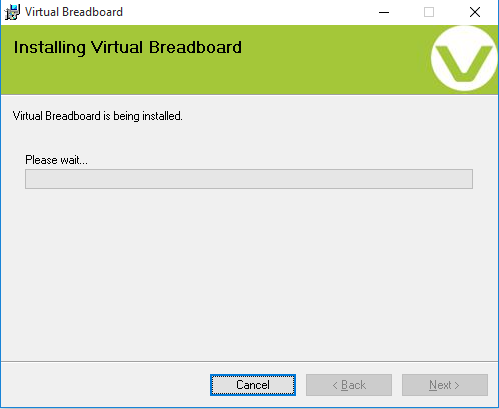
\includegraphics[width=.75\textwidth]{figures/VBB/prosesinstallasi.png}
            \caption{Ini adalah Proses Installasi}\label{fig:prosesinstallasi}
            \end{figure}
        \item Proses installasi selesai, seperti pada gambar \ref{fig:installasiselesai}
            \begin{figure}[!htbp]
            \centering
            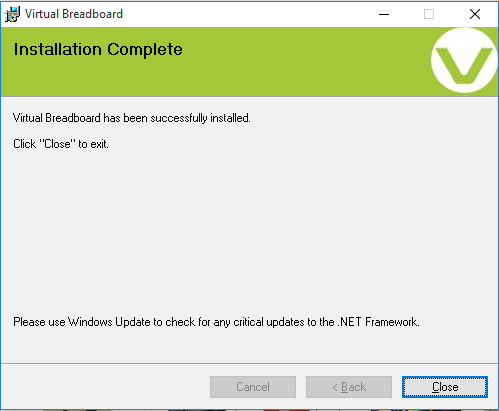
\includegraphics[width=.75\textwidth]{figures/VBB/installasiselesai.png}
            \caption{Ini adalah Proses Installasi Telah Selesai}\label{fig:installasiselesai}
            \end{figure}
        \end{enumerate}
    \item Installasi IDE(\textit{Integrated Development Envyronment})
            \begin{enumerate}
              \item Download installer IDE
            \item Double-click installer vbb,seperti pada gambar \ref{fig:installer}
                \begin{figure}[!htbp]
                \centering
                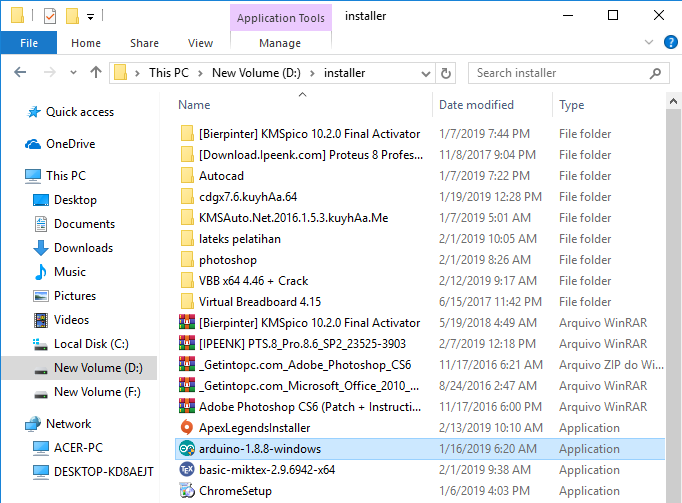
\includegraphics[width=.75\textwidth]{figures/IDE/installer.png}
                \caption{Ini adalah installer}\label{fig:installer}
                \end{figure}
            \item Maka akan tampil seperti gambar \ref{fig:agreement}
                \begin{figure}[!htbp]
                \centering
                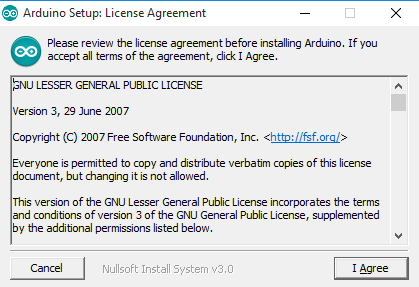
\includegraphics[width=.75\textwidth]{figures/IDE/agreement.png}
                \caption{Ini adalah Halaman Agreement}\label{fig:agreement}
                \end{figure}
            \item Pilih \textbf{Agree} maka akan muncul halaman \textit{Installation Options} seperti pada gambar \ref{fig:option}
                \begin{figure}[!htbp]
                \centering
                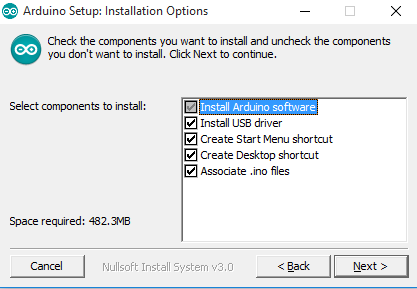
\includegraphics[width=.75\textwidth]{figures/IDE/option.png}
                \caption{Ini adalah Halaman Installation Options}\label{fig:option}
                \end{figure}
            \item Kemudian tekan tombol next, maka akan muncul halaman pemilihan direktori penyimpanan seperti pada gambar \ref{fig:dir}
                \begin{figure}[!htbp]
                \centering
                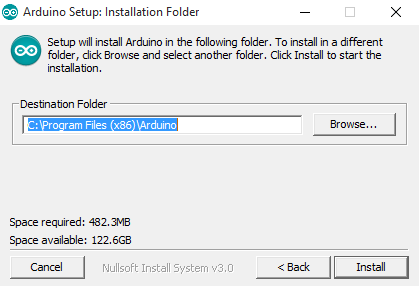
\includegraphics[width=.75\textwidth]{figures/IDE/dir.png}
                \caption{Ini adalah Halaman Pemilihan Direktori}\label{fig:dir}
                \end{figure}
            \item Kemudian tekan tombol install, maka proses installasi dimulai seperti pada gambar \ref{fig:installing}
                \begin{figure}[!htbp]
                \centering
                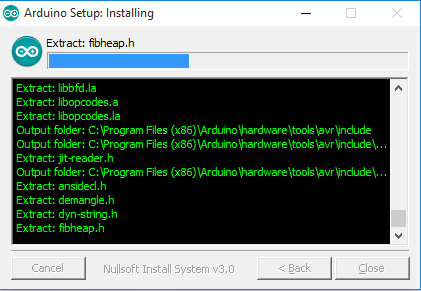
\includegraphics[width=.75\textwidth]{figures/IDE/installing.png}
                \caption{Ini adalah Proses Installasi IDE}\label{fig:installing}
                \end{figure}
            \item Proses installasi selesai, seperti pada gambar \ref{fig:complete}
                \begin{figure}[!htbp]
                \centering
                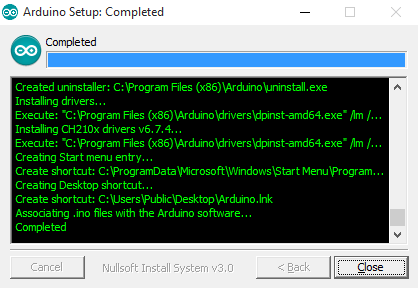
\includegraphics[width=.75\textwidth]{figures/IDE/complete.png}
                \caption{Ini adalah Proses Installasi Telah Selesai}\label{fig:complete}
                \end{figure}
            \end{enumerate}
    \item \textit{Coming Soon}
\end{enumerate}
